\documentclass[12pt,a4paper]{report}

%adjust your page margins here
\usepackage[top=0.70in, bottom=0.70in, left=0.8in,right=0.80in]{geometry} % setting the page alignment with this package
\usepackage[pdftex]{graphicx} %for embedding images
\usepackage[%dvips, % commented for pdflatex
bookmarks,  colorlinks=false]{hyperref} %for creating links in the pdf version and other additional pdf attributes, no effect on the printed document
\hypersetup{%
    pdfborder = {0 0 0}
}
\usepackage[final]{pdfpages} %for embedding another pdf, remove if not required
\usepackage{float} %used for figure placement with H as a parameter
\usepackage{hyperref}
\usepackage{pslatex} % for times new roman, old package, but works
\usepackage{array} % for making text bold in table
\usepackage{setspace}
\usepackage{float}
\usepackage{enumerate}
\usepackage{longtable}

\usepackage[font=small,labelfont=bf]{caption}
\def\figurename{\textbf{Figure }}

\usepackage{listings}
\usepackage{color}

\definecolor{dkgreen}{rgb}{0,0.6,0}
\definecolor{gray}{rgb}{0.5,0.5,0.5}
\definecolor{mauve}{rgb}{0.58,0,0.82}
 
\lstset{ %
  language=Java,                % the language of the code
  basicstyle=\footnotesize,           % the size of the fonts that are used for the code
  numbers=left,                   % where to put the line-numbers
  numberstyle=\large\color{gray},  % the style that is used for the line-numbers
  stepnumber=1,                   % each line is numbered
  numbersep=8pt,                  % how far the line-numbers are from the code
%   Font Size=8pt,
  backgroundcolor=\color{white},      % choose the background color. You must add \usepackage{color}
  showspaces=false,               % show spaces adding particular underscores
  vspace=1cm,
  showstringspaces=false,         % underline spaces within strings
  showtabs=false,                 % show tabs within strings adding particular underscores
  frame=single,                   % adds a frame around the code
  rulecolor=\color{black},        % if not set, the frame-color may be changed on line-breaks within not-black text (e.g. commens (green here))
  tabsize=2,                      % sets default tabsize to 2 spaces
  captionpos=b,                   % sets the caption-position to bottom
  breaklines=true,                % sets automatic line breaking
  breakatwhitespace=true,        % sets if automatic breaks should only happen at whitespace
  title=\lstname,                   % show the filename of files included with \lstinputlisting;
                                  % also try caption instead of title
  keywordstyle=\color{blue},          % keyword style
  commentstyle=\color{dkgreen},       % comment style
  stringstyle=\color{mauve},         % string literal style
  escapeinside={\%*}{*)},            % if you want to add a comment within your code
  morekeywords={*,...}               % if you want to add more keywords to the set
}

%Page Border
\usepackage{pgf}
\usepackage{pgfpages}

\pgfpagesdeclarelayout{boxed}
{
  \edef\pgfpageoptionborder{0pt}
}
{
  \pgfpagesphysicalpageoptions
  {%
    logical pages=1,%
  }
  \pgfpageslogicalpageoptions{1}
  {
    border code=\pgfsetlinewidth{3pt}\pgfstroke,%
    border shrink=\pgfpageoptionborder,%
    resized width=.95\pgfphysicalwidth,%
    resized height=.95\pgfphysicalheight,%
    center=\pgfpoint{.5\pgfphysicalwidth}{.5\pgfphysicalheight}%
  }%
}
\pgfpagesuselayout{boxed}
\setlength{\parindent}{1cm}
%GLOBAL SETTINGS OVER, DOCUMENT BEGINS
\begin{document}
\renewcommand\bibname{References}
\lhead{ }

%FROM HERE YOUR PAGES START GETTING ADDED

% includes the cover page
\newpage
\begin{center}
\thispagestyle{empty}
\LARGE{\textbf{MOTILAL    NEHRU   NATIONAL   INSTITUTE   OF TECHNOLOGY \\ \centering{ ALLAHABAD,INDIA-211004 \\ }}}\\[0.14cm] 
\vspace{1.0cm}

\includegraphics[scale=0.2]{project/images/MNNIT}\\\vspace{1cm}
\Large{\textbf{A PROJECT REPORT\\ \large{ON}}}\\[0.7cm]
\LARGE{ \textsc {\textbf{``TYPING TEST''}}}\\[0.5cm]
\vspace{0.5cm}
\Large{\textbf{\\Submitted to}}
\LARGE{\textbf{\\MOTILAL NEHRU NATIONAL  INSTITUTE OF TECHNOLOGY ALLAHABAD \\}}
\vspace{1cm}
\Large{\textbf{\\In Partial fulfillment  of the Requirement for the Award of\\}}
\Large{\textbf{\\MASTER OF
COMPUTER APPLICATION from MNNIT ALLHABAD for the academic year 2016-2019.\\}}
\vspace{1cm}
\Large{\textbf{\\SUBMITED}}\\[0.1cm]
\Large{\textbf{\\BY}}\\[0.5cm]
\begin{table}[h]
\centering
\Large{
\begin{tabular}{>{\bfseries}lc>{\bfseries}r}
AADITYA SUPRIYO & & 2016CA90\\AAKRITI GUPTA & & 2016CA55\\ABHISHEK GUPTA & & 2016CA29\\ABHISHEK KUMAR & & 2016CA04\\
\end{tabular}}
\end{table}
\vspace{0.5cm}
\large{\textbf{UNDER THE GUIDANCE OF}}\\
\LARGE{\textbf{PROF.  M.M GORE}}\\
\vspace{0.5cm}
\large{\textbf{DEPARTMENT OF COMPUTER SCIENCE AND ENGINEERING}}\\
\Large{\textbf{MNNIT}}\\
\large{\textbf{ALLAHABAD - 211004}}
\large{\textbf{\\2018-2019}}\\
\vspace{1cm}
\newpage
\end{center}
\newpage

\input{project/title.tex}
\newpage

% includes the certificate page
\input{project/certificate.tex} 
\newpage

% includes the acknowledgements page
\begin{center}
\thispagestyle{empty}
\LARGE{\textbf{Acknowledgements}}\\[1cm]
\end{center}
\linespread{1.13}
\large{\paragraph{}We are profoundly grateful to \textbf{Prof. M.M Gore } for his expert guidance
and continuous encouragement throughout to see that this project rights its
target since its commencement to its completion.}
\large{\paragraph{}We would like to express deepest appreciation towards \textbf{Prof. A.K. SINGH}, 
Head of Department of Computer Science and  Engineering and \textbf{Prof. M.M Gore}, Project Coordinator whose
invaluable guidance supported us in completing this project.}
\large{\paragraph{}At last we must express our sincere heartfelt gratitude to all the staff members
of Computer Engineering Department who helped me directly or indirectly during this course of work.}
\begin{flushright}
{
Aaditya Supriyo\\
Aakriti Gupta\\
Abhishek Gupta\\
Abhishek Kumar
}
\end{flushright}
\newpage
 
\newpage

\begin{center}
\thispagestyle{empty}
\vspace{2cm}
\LARGE{\textbf{ABSTRACT}}\\[1.0cm]
\end{center}
\thispagestyle{empty}
\large{\paragraph{}
This is a advanced PHP,HTML,CSS,Bootstrap Typing Test system that will allow you to place a table and a few blocks of code on your website and get a detailed statistical information on your user's typing ability, including:

    1)Words Per Minute (WPM)
    2)Accuracy Percentage Rating
    3)Total Words Typed
    4)Good Words / Bad Words Typed (Errors)
    5)Time Taken to Complete
    6)More as needed.
    You can check your typing speed and accuracy online. Compare it with other results in the rankings and increase it using Ratatype. We measure your typing speed in WPM (words per minute). It is a calculation of how fast you type words with no typos. By the "word" we mean an average of 5 characters including spaces. We measure gross speed in our typing test. \\
}
\textbf{ \Large{ \\ Keywords:} } Typing Test, Words Per Minute(WPM),Errors,Accuracy. % adds the Research Methodology page
\newpage

%TABLE OF CONTENTS AND LIST OF FIGURES ARE AUTOMATICALLY ADDED BY FOLLOWING COMMANDS
%ADD FIGURE OF TABLES IF YOU NEED TO, CHECK DOCUMENTATION
\pagenumbering{roman} %numbering before main content starts


%To reset the Header & Footer for TOC and LOF
\pagestyle{empty}
\addtocontents{toc}{\protect\thispagestyle{empty}}
\tableofcontents % adds Index Page

\addtocontents{lof}{\protect\thispagestyle{empty}}
\listoffigures % adds List of Figures
\cleardoublepage

%And reset back the settings we choose for Header and Footer

\newpage
\pagenumbering{arabic} %reset numbering to normal for the main content

\chapter{Introduction}
\section{
About TYPING TEST}
\large{ \paragraph{
}
Today Typing Test has become a fast growing examination method because of its speed and accuracy. It is also needed less manpower to execute the test. Almost all organizations now-a-days, are conducting typing test to test the speed of typing. Organizations can also easily check the performance of the student that they give in an test. As a result of this, organizations are releasing results in less time. It also helps the environment by saving paper.
According to today’s requirement, typing test project in php is very useful.
}

\section{About The Project}
 \large{\paragraph{}
  The project \textbf{"Typing Test"} is a Web Application which provides facility to conduct online test anytime anywhere.It saves time as it allows number of students to give the test at a 
time  and  displays  the  results  as  the  test  gets  over, so  no need  to wait for the result. It is automatically generated by the server. Administrator has a privilege to create, modify and delete the test and its particular content. User can register, login and give the test with his specific id, and can see the results as well.

In Typing Test examine get their user id and password. This id is already saved in the examination server. When examine login to the server he/she get his/her profile already register. On the certain time examine gets the message to start the examination. All inputs  given by examine are saved into the server with his/her profile information. Online examination system also allows to correct the spellings if the examine needed to change any spelling in the examination time duration, however, after the time duration any change will not allow. This also makes checking the answer easy and error proof as computers are more accurate than man and provide fast results too. Php is a web base language so we can create Typing Test in PHP.
 }
 % adds the introduction page
% \chapter{Literature Survey}
% \section{SECTION NAME}
% \paragraph{}WRITE HERE
% \begin{enumerate}[a. ]
%  \item ITEM 1
%  \item ITEM 2
%  \item ITEM 3
% \end{enumerate} % adds the Literature Survey page
\chapter{Software Requirements Specification}
\section{Software Requiremnts}
\begin{center}
  \begin{tabular}{ | l | c |}
    \hline \hline
    \textbf{COMPONENTS} &  \textbf{MINIMUM} \\ \hline
    OPERATING SYSTEM & Windos 7/8/10(32 or 64 bit) \\ \hline
    IDE &  WAMP SERVER \\ \hline
    FRONT-END & HTML,CSS,BOOTSTRAP \\ \hline
    BACK-END & PHP \\ \hline
    \hline
  \end{tabular}\\ 
  \vspace{1cm}
  Table 2.1.1
\end{center}
    
\section{Hardware Requirements}
\begin{center}
  \begin{tabular}{ | l | c |}
    \hline \hline
    \textbf{COMPONANTS} &  \textbf{MINIMUM} \\ \hline
    RAM & 2GB \\ \hline
    DISK &  3GB(1GB additional)  \\ \hline
    MONITOR & 640 X 480 px \\ \hline
    \hline
  \end{tabular}\\ \\
  \vspace{1cm}
  Table 2.2.1
\end{center}
\chapter{Requirement Analysis}
\section{SECTION NAME}
\paragraph{} .
\chapter{System Design}
\section{SECTION 1}
\begin{center}
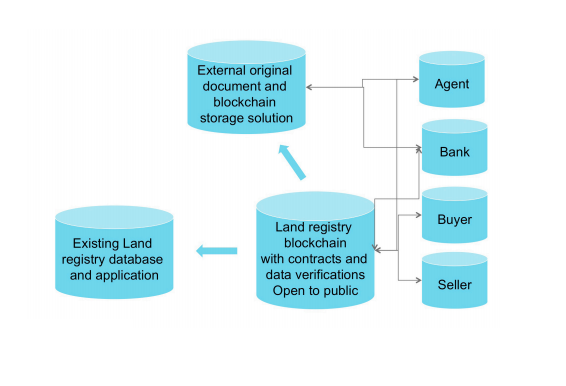
\includegraphics[scale=1.2]{project/images/dbms2}\\
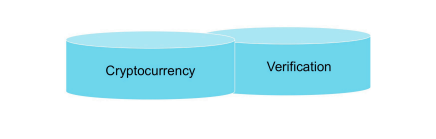
\includegraphics[scale=1.2]{project/images/dbms3}
\end{center}
\section{SECTION 2}
\begin{center}
 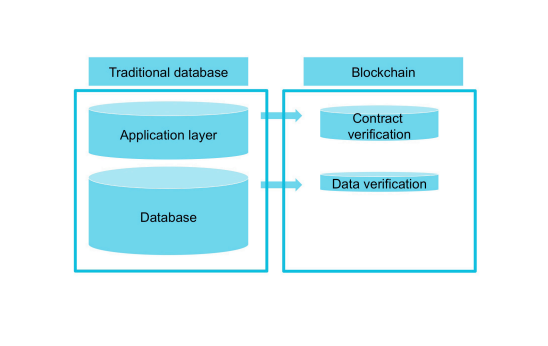
\includegraphics[scale=1.2]{project/images/dbms}
 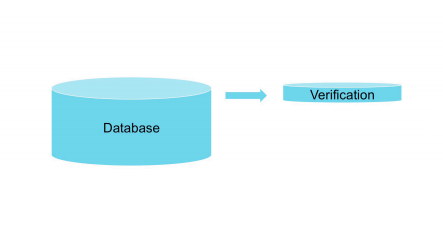
\includegraphics[scale=1.2]{project/images/dbms4}
 \end{center}
\chapter{System Testing}
\paragraph{}
\section{Test Cases and Test Results}
\begin{longtable}{ | p{1cm} | p{3.5cm} | p{4cm} | p{4cm} | p{4cm} |}
      \hline
      \textbf{Test ID} & \textbf{Test Case Title} & \textbf{Test Condition} & \textbf{System Behavior} & \textbf{Expected Result}\\
      \hline
      T01 & Register Land & Owner Exist And Valid User & Transaction Successful & Successfully  Registered\\
      \hline
       T02 & Register Land & Owner Exist and Not Valid User & Transaction Failed& failure\\
      \hline T03 & Search Land & Owner Exist and Land Exist & Transaction Successful & Successfully searched\\
      \hline
       T04& Register Land & Owner Not Exist and NOT valid User& Transaction Failed & Failure \\
      \hline
       T05& Register Land & Owner Not Exist and valid User& Transaction successful & Successfully Registered \\
      \hline
       T06& Search Land & Owner Exist and Land Not Exist&Land Not Found& Failure \\
      \hline 
      T06& Search Land & Owner Not Exist and Land Not Exist&Transaction Failed& Failure \\
      \hline 
\end{longtable}

\textbf{Note: Testing performed manually}
\chapter{Project Planning}
\section{SECTION 1}
\paragraph{} WRITE HERE.

\chapter{Implementation}
\paragraph{}WRITE HERE, PARAGRAPH 1.

\begin{lstlisting}
pragma solidity ^0.4.0;

contract Registry {
    struct Detail {
        string ownerName;
        string dateOfRegistry;
        uint32 khasraNumber;
    }
    address private contractOwner;
    mapping(uint64 => Detail) registryList;
    
    function Registry() public {
        contractOwner = msg.sender;
    }
    function isOwnerOfContract() view public returns (bool) {
        return msg.sender == contractOwner;
    }
    function newRegistry(uint64 hash, uint32 khasraNumber, string name, string dateOfRegistry) public returns (bool) {
        if(isOwnerOfContract()) {
            registryList[hash].ownerName = name;
            registryList[hash].khasraNumber = khasraNumber;
            registryList[hash].dateOfRegistry = dateOfRegistry;
            return true;
        }
        return false;
    }
    
    function getRegistry(uint64 hash) view public returns (string, string, uint32) {
        return (registryList[hash].ownerName, registryList[hash].dateOfRegistry, registryList[hash].khasraNumber);
    }
}
\end{lstlisting}
\paragraph{} write paragraph here 2
\begin{lstlisting}
 const express = require('express');
const Web3 = require('web3');
const hbs = require('hbs');
const fs = require('fs');
const parser = require('body-parser');
const sha = require('sha256');

const pathToSolidity = __dirname +'/SolidityCode/';
var urlencodedParser = parser.urlencoded({ extended: true });
const app = express();
app.use(urlencodedParser);

app.set('view engine', 'hbs');


web3 = new Web3(new Web3.providers.HttpProvider("http://localhost:8545"));

abiDefinition = JSON.parse(fs.readFileSync(pathToSolidity +'interface.json'));
RegistryContract = web3.eth.contract(abiDefinition);

contractInstance = RegistryContract.at(fs.readFileSync(pathToSolidity +'contractAddress').toString());


app.get('/', (req, res) => {
	res.render('index');
});

app.post('/registerLand', (req, res) => {
	var name = req.body.owner;
	var city = req.body.city;
	var area = req.body.area;
	var khasraNumber = req.body.khasraNumber;
	var date = req.body.date;
	var transactionId = contractInstance.newRegistry(parseInt(sha(city +area +khasraNumber)), khasraNumber, name, date, {from: web3.eth.accounts[0]});
	console.log(transactionId);
	res.render('index');
});

app.post('/getLand', (req, res) => {
	var city = req.body.city;
	var area = req.body.area;
	var khasraNumber = req.body.khasraNumber;
	var result = contractInstance.getRegistry.call(parseInt(sha(city +area +khasraNumber)));
	res.send(result);
	console.log(result);
});


app.listen(3000, () => {
	console.log("Listening on port 3000");
});
\end{lstlisting}
\paragraph{}WRITE HERE, PARAGRAPH 2.

\begin{lstlisting}
const fs = require('fs');
const sol = require('solc');
const Web3 = require('web3');

const pathToSolidity = __dirname +'/SolidityCode/';
code = fs.readFileSync(pathToSolidity +'code.sol').toString();

compiledCode = sol.compile(code);
web3 = new Web3(new Web3.providers.HttpProvider("http://localhost:8545"));


abiDefinition = JSON.parse(compiledCode.contracts[':Registry'].interface);
Registry = web3.eth.contract(abiDefinition);

byteCode = '0x' +compiledCode.contracts[':Registry'].bytecode;
interface = compiledCode.contracts[':Registry'].interface;
dc = Registry.new([], {data: byteCode, from: web3.eth.accounts[0], gas: 4700000});
// console.log('Address is ', dc.address);
fs.writeFileSync(pathToSolidity +'interface.json', interface);
if(dc != undefined)
	fs.writeFileSync(pathToSolidity +'contractAddress', dc.address);
console.log('Code Deployed');
\end{lstlisting}
\paragraph{} This is INTERFACE Code 
\begin{lstlisting}
[{"constant":false,"inputs":[{"name":"hash","type":"uint64"},
{"name":"khasraNumber","type":"uint32"},{"name":"name","type":"string"},
{"name":"dateOfRegistry","type":"string"}],"name":"newRegistry",
"outputs":[{"name":"","type":"bool"}],"payable":false,
"stateMutability":"nonpayable","type":"function"},{"constant":true,"inputs":[],
"name":"isOwnerOfContract","outputs":[{"name":"","type":"bool"}],
"payable":false,"stateMutability":"view","type":"function"},
{"constant":true,"inputs":[{"name":"hash","type":"uint64"}],
"name":"getRegistry","outputs":[{"name":"","type":"string"},
{"name":"","type":"string"},{"name":"","type":"uint32"}],
"payable":false,"stateMutability":"view","type":"function"},
{"inputs":[],"payable":false,"stateMutability":"nonpayable",
"type":"constructor"}]
\end{lstlisting}
\paragraph{} NODE JS PROGRAM ...
\begin{lstlisting}
<!DOCTYPE html>
<!DOCTYPE html>
<html>
<head>
	<title>Block-chain</title>
	<link rel="stylesheet" href="https://maxcdn.bootstrapcdn.com/bootstrap/4.0.0/css
	/bootstrap.min.css" integrity="sha384-Gn5384xqQ1aoWXA+
	058RXPxPg6fy4IWvTNh0E263XmFcJlSAwiGgFAW/dAiS6JXm" crossorigin="anonymous">

</head>
<body>
	<H1 align= "center" style="margin-top: 24px;">Welcome to block chain</H1>
	<div class="container">
		<div class="row">
			<div class="col-lg-6" align="center" style="margin-top: 16px">
		<h3>Register Land</h3>
		<form class="jumbotron" action="registerLand" method="post" style="max-width: 400px">
			<input class="form-control" type="text" name="owner" placeholder="Owner" maxlength="20"><br>
			<input class="form-control" type="text" name="city" placeholder="City Name" maxlength="20"><br>
			<input class="form-control" type="text" name="area" placeholder="Area Name" maxlength="20"><br>
			<input class="form-control" type="number" name="khasraNumber" placeholder="Khasra Number" maxlength="20"><br>
			<input class="form-control" type="date" name="date" placeholder="Date of Registry" maxlength="10"><br>
			<button type="Submit" class="btn btn-danger form-control">Submit</button>
		</form>
	</div>
	<div class="col-lg-6" align="center" style="margin-top: 16px">
		<h3>Search Land</h3>
		<form class="jumbotron" action="getLand" method="post"
		style="max-width: 400px">
			<input class="form-control" type="text" name="city" placeholder="City Name" maxlength="20"><br>
			<input class="form-control" type="text" name="area" placeholder="Area Name" maxlength="20"><br>
			<input class="form-control" type="number" name="khasraNumber" placeholder="Khasra Number" maxlength="20"><br>
			<button type="Submit" class="btn btn-success form-control">Search</button>
		</form>
	</div>
		</div>
	</div>
	
	<script src="https://code.jquery.com/jquery-3.2.1.slim.min.js" integrity="sha384-KJ3o2DKtIkvYIK3UENzmM7KCkRr/
	rE9/
	Qpg6aAZGJwFDMVNA/GpGFF93hXpG5KkN" crossorigin="anonymous"></script>
<script src="https://cdnjs.cloudflare.com/ajax/libs/
popper.js/1.12.9/umd/popper.min.js" integrity="sha384-ApNbgh9B+Y1QKtv3Rn7W3mgPxhU9K/
ScQsAP7hUibX39j7fakFPskvXusvfa0b4Q" crossorigin="anonymous"></script>
<script src="https://maxcdn.bootstrapcdn.com/bootstrap/4.0.0/js/bootstrap.min.js" integrity="sha384-JZR6Spejh4U02d8jOt6vLEHfe/
JQGiRRSQQxSfFWpi1MquVdAyjUar5+76PVCmYl" crossorigin="anonymous"></script>
</body>
</html>
\end{lstlisting}

\paragraph{} This Is ganache CLI CONTENT
\begin{lstlisting}
@IF EXIST "%~dp0\node.exe" (
  "%~dp0\node.exe"  "%~dp0\..\ganache-cli\build\cli.node.js" %*
) ELSE (
  @SETLOCAL
  @SET PATHEXT=%PATHEXT:;.JS;=;%
  node  "%~dp0\..\ganache-cli\build\cli.node.js" %*
)
\end{lstlisting}

\paragraph{} This is the Manual to Run Application
\begin{lstlisting}
Install node js 

npm install //to install all dependencies
npm install ganache-cli //to install ganache blockchain simulator

 Go through the following steps to deploy contract and to use the Application
	1.Open terminal in project directory and type "node_modules/.bin/ganache-cli" 
	2.Open new terminal in project directory and type "node deployecode.js"
	3.Copy the contract address obtained in "SolidityCode/contractAddress" file
	4.Type the command "node app.js" in terminal

Open browser and goto address : "localhost:3000"  
\end{lstlisting}
\newpage

 % adds the Project Design
\chapter{Screenshots of Project}
\section{SECTION NAME}
\vspace{2cm}
\begin{figure}[H]
  \centering
    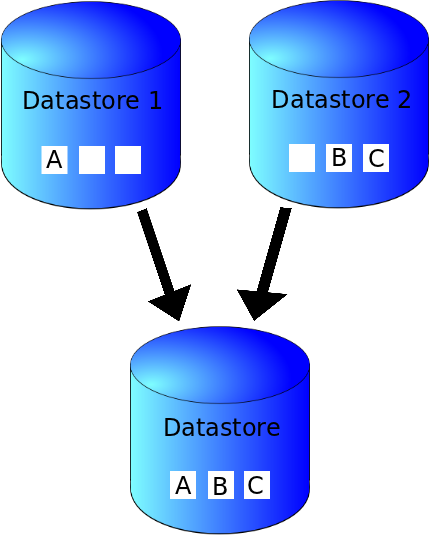
\includegraphics[height= 11cm, width=17cm]{project/images/data-sync}
\end{figure}
\newpage
\begin{figure}[H]
  \centering
    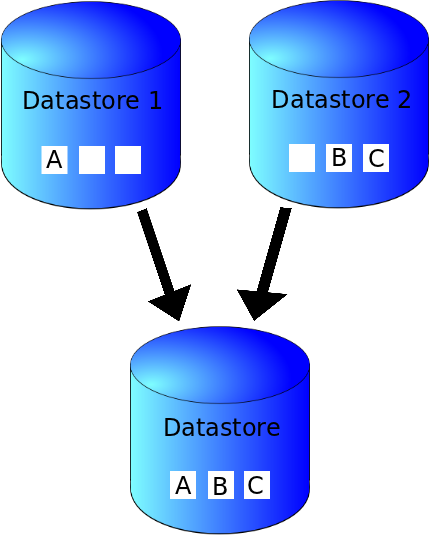
\includegraphics[height= 11cm, width=17cm]{project/images/data-sync}
\end{figure}
\vspace{1cm}
\begin{figure}[H]
  \centering
    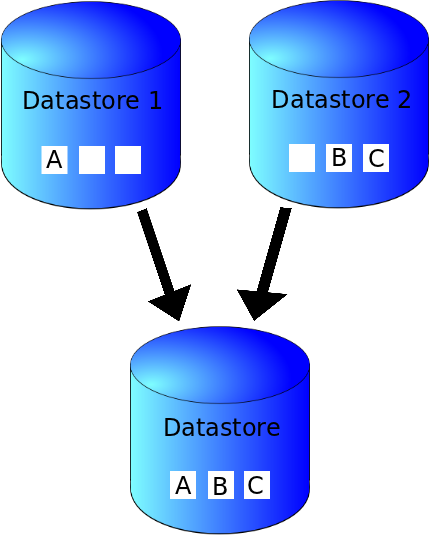
\includegraphics[height= 11cm, width=17cm]{project/images/data-sync}
\end{figure}
\chapter{Conclusion and Future Scope}
\section{Conclusion}
\paragraph{}WRITE HERE.
\section{Future Scope}
\paragraph{}WRITE HERE.
\begin{itemize}
 \item ITEM 1
 \item ITEM 2
 \item ITEM 3
\end{itemize} % adds the Scheduling and Planning page
\addcontentsline{toc}{chapter}{References}
\begin{thebibliography}{99}
\bibitem{WRITE A SHORT-NAME WITHOUT SPACE} \emph{NAME OF IEEE PAPER}; NAME OF AUTHORS
\bibitem{WRITE A SHORT-NAME WITHOUT SPACE} \url{http://EXAMPLE.com}
\end{thebibliography} % adds the References page

\end{document}